\documentclass[11pt]{article}
\usepackage[a4paper,margin=25mm,marginparwidth=20mm,marginparsep=10pt]{geometry}
\usepackage{fontspec}
\usepackage{amsmath,amssymb,mathtools}
\usepackage{unicode-math}
\usepackage[normalem]{ulem}
\usepackage{graphicx,xcolor,tikz,tikz-cd,pdflscape,needspace}
\usetikzlibrary{calc,decorations.pathmorphing,decorations.pathreplacing,arrows.meta,shapes.geometric}
\usepackage{newunicodechar,luacode,xurl}
\usepackage[hidelinks,unicode]{hyperref}
\setmainfont{Latin Modern Roman}
\setmathfont{Latin Modern Math}
\setmathfont{STIX Two Math}[range={"27CB,"27CD}]
\newfontfamily\cyrfont{STIX Two Text}[Scale=MatchLowercase]
\newunicodechar{А}{{\cyrfont\char"0410}}
\newunicodechar{Б}{{\cyrfont\char"0411}}
\newunicodechar{В}{{\cyrfont\char"0412}}
\newunicodechar{Г}{{\cyrfont\char"0413}}
\newunicodechar{Д}{{\cyrfont\char"0414}}
\newunicodechar{Е}{{\cyrfont\char"0415}}
\newunicodechar{Ж}{{\cyrfont\char"0416}}
\newunicodechar{З}{{\cyrfont\char"0417}}
\newunicodechar{И}{{\cyrfont\char"0418}}
\newunicodechar{Й}{{\cyrfont\char"0419}}
\newunicodechar{К}{{\cyrfont\char"041A}}
\newunicodechar{Л}{{\cyrfont\char"041B}}
\newunicodechar{М}{{\cyrfont\char"041C}}
\newunicodechar{Н}{{\cyrfont\char"041D}}
\newunicodechar{О}{{\cyrfont\char"041E}}
\newunicodechar{П}{{\cyrfont\char"041F}}
\newunicodechar{Р}{{\cyrfont\char"0420}}
\newunicodechar{С}{{\cyrfont\char"0421}}
\newunicodechar{Т}{{\cyrfont\char"0422}}
\newunicodechar{У}{{\cyrfont\char"0423}}
\newunicodechar{Ф}{{\cyrfont\char"0424}}
\newunicodechar{Х}{{\cyrfont\char"0425}}
\newunicodechar{Ц}{{\cyrfont\char"0426}}
\newunicodechar{Ч}{{\cyrfont\char"0427}}
\newunicodechar{Ш}{{\cyrfont\char"0428}}
\newunicodechar{Щ}{{\cyrfont\char"0429}}
\newunicodechar{Ъ}{{\cyrfont\char"042A}}
\newunicodechar{Ы}{{\cyrfont\char"042B}}
\newunicodechar{Ь}{{\cyrfont\char"042C}}
\newunicodechar{Э}{{\cyrfont\char"042D}}
\newunicodechar{Ю}{{\cyrfont\char"042E}}
\newunicodechar{Я}{{\cyrfont\char"042F}}
\newunicodechar{а}{{\cyrfont\char"0430}}
\newunicodechar{б}{{\cyrfont\char"0431}}
\newunicodechar{в}{{\cyrfont\char"0432}}
\newunicodechar{г}{{\cyrfont\char"0433}}
\newunicodechar{д}{{\cyrfont\char"0434}}
\newunicodechar{е}{{\cyrfont\char"0435}}
\newunicodechar{ж}{{\cyrfont\char"0436}}
\newunicodechar{з}{{\cyrfont\char"0437}}
\newunicodechar{и}{{\cyrfont\char"0438}}
\newunicodechar{й}{{\cyrfont\char"0439}}
\newunicodechar{к}{{\cyrfont\char"043A}}
\newunicodechar{л}{{\cyrfont\char"043B}}
\newunicodechar{м}{{\cyrfont\char"043C}}
\newunicodechar{н}{{\cyrfont\char"043D}}
\newunicodechar{о}{{\cyrfont\char"043E}}
\newunicodechar{п}{{\cyrfont\char"043F}}
\newunicodechar{р}{{\cyrfont\char"0440}}
\newunicodechar{с}{{\cyrfont\char"0441}}
\newunicodechar{т}{{\cyrfont\char"0442}}
\newunicodechar{у}{{\cyrfont\char"0443}}
\newunicodechar{ф}{{\cyrfont\char"0444}}
\newunicodechar{х}{{\cyrfont\char"0445}}
\newunicodechar{ц}{{\cyrfont\char"0446}}
\newunicodechar{ч}{{\cyrfont\char"0447}}
\newunicodechar{ш}{{\cyrfont\char"0448}}
\newunicodechar{щ}{{\cyrfont\char"0449}}
\newunicodechar{ъ}{{\cyrfont\char"044A}}
\newunicodechar{ы}{{\cyrfont\char"044B}}
\newunicodechar{ь}{{\cyrfont\char"044C}}
\newunicodechar{э}{{\cyrfont\char"044D}}
\newunicodechar{ю}{{\cyrfont\char"044E}}
\newunicodechar{я}{{\cyrfont\char"044F}}
\newunicodechar{≃}{\ensuremath{\simeq}}
\newattribute\LMattr
\newcount\LMform
\newcount\LMinApp
\LMform=2
\LMinApp=0
\newcommand\LMlanguage{en}
\newcommand\LMcotename{}
\newcommand\LMcote[1]{\gdef\LMcotename{#1}}
\newcommand\LMnotelabel{Marginal note}
\newcommand\LMappheading{Apparatus for this scan}
\newcommand\LMdoubtheading{Uncertainty retained from cancelled passages}
\newcommand\LMmanuscriptlabel{Manuscript}
\newcommand\LMcorrectedlabel{Text}
\newcommand\LMreasonlabel{Reason}
\newcommand\LMomittedlabel{omitted}
\newcommand\LMinsertedlabel{insertion integrated}
\newcommand\LMlayoutlabel{Diagram continued on the landscape page}
\newcommand\LMvarref[1]{\ifmmode\else\ifinner\else\textsuperscript{\textcolor{gray}{\LMreftext{#1}}}\fi\fi}
\newcommand\LMreftext[1]{\directlua{LM.reftext("\luaescapestring{#1}")}}
\newcommand\var[4]{\ifcase\LMform #1\or #2\ifnum\LMinApp=0\LMvarref{#4}\fi\or #2\fi}
\newcommand\LMadded[1]{{\color{teal}#1}}
\newcommand\deleted[1]{{\color{gray}#1}}
\newcommand\inserted[1]{{\color{teal}#1}}
\newcommand\LMarchivefooter[3]{#2}
\newcommand\LMsourceid{}
\newcommand\LMsourceMark[2]{{\def\LMsourceid{#1}#2}}
\newcommand\LMmark[1]{\directlua{LM.mark("#1",tex.inputlineno)}}
\newcommand\unsure[1]{{\color{blue}\LMmark{unsure}#1}}
\newcommand\illegible[1]{{\LMmark{illegible}\textcolor{red}{[illeg.~#1]}}}
\newcommand\LMuncertaindeletion[1]{{\color{blue}\LMmark{cancelled-anchor}\ensuremath{\dagger}}}
\newcommand\LMdoubtcopy[1]{{\color{blue}\LMmark{residual-unsure}#1}}
\newcommand\LMdoubtdata[1]{}
\newcommand\LMcancelledDoubts[1]{\ifnum\LMform=2{\color{blue}\LMmark{cancelled-anchor}\ensuremath{\dagger}}\fi}
\newcommand\scanpage[1]{%
 \par\LMflushnotes\LMflushpages\smallskip\directlua{LM.at("\luaescapestring{\LMcotename}","\luaescapestring{\detokenize{#1}}")}%
 \ifnum\LMform=2\noindent\marginpar{\footnotesize\raggedright\LMmark{scan}\textcolor{gray}{[scan #1]}}%
 \else\noindent{\footnotesize\LMmark{scan}\textcolor{gray}{[scan #1]}}\par\nobreak\fi}
\newcommand\mspage[1]{\ifnum\LMform=2\ifinner\LMqueuepage{#1}\else\marginpar{\footnotesize\raggedright\textcolor{gray}{[p.~#1]}}\fi\else{\footnotesize\textcolor{gray}{[p.~#1]}}\ \fi}
\newcommand\diagram[1]{\ifmmode\vcenter{\hbox{#1}}\else\ifinner #1\else\par\begin{center}#1\end{center}\par\LMflushnotes\LMflushpages\fi\fi}
\let\figure\relax\newcommand\figure[1]{\ifmmode\vcenter{\hbox{#1}}\else\ifinner #1\else\par\begin{center}#1\end{center}\par\LMflushnotes\LMflushpages\fi\fi}
\newcommand\LMmathnotice[1]{\par\noindent{\footnotesize\color{gray}[\ensuremath{\hookrightarrow}\ #1]}\par}
\newcommand\LMlayoutnotice[1]{\par\noindent{\footnotesize\color{gray}[\LMlayoutlabel; #1]}\par}
\tolerance=1200
\emergencystretch=3em
\tracinglostchars=3
\hfuzz=0pt
\vfuzz=0pt
\raggedbottom
\setcounter{tocdepth}{1}
\setlength\parindent{1.3em}
\setlength\parskip{1.5pt plus 1pt}
\allowdisplaybreaks[2]
\begin{luacode*}
-- Marked passages are linked at shipout, including paragraphs and mathematics.
-- No node, line, display or font is scaled by this code.
LM = {measure=false, maxw=0, markers={}, links=0, pages=0, scanmap={}, trial_overfull=0, shortnotes=0, blocknotes=0}
local F=LM
local A=luatexbase.registernumber('LMattr')
local HLIST,VLIST,GLUE,KERN,WHATSIT,GLYPH,PENALTY,MATH = node.id('hlist'),node.id('vlist'),node.id('glue'),node.id('kern'),node.id('whatsit'),node.id('glyph'),node.id('penalty'),node.id('math')
local STARTLINK,ENDLINK,ACTION=node.subtype('pdf_start_link'),node.subtype('pdf_end_link'),node.subtype('pdf_action')
local inert={[GLUE]=true,[KERN]=true,[PENALTY]=true,[WHATSIT]=true,[MATH]=true}
function F.at(cote,scan)
 F.cote=cote;F.scan=tonumber(string.match(scan,'^%s*(%d+)')) or 0
end
F.by_source={}
function F.mark(kind,line)
 if F.measure or not F.cote or not F.scan or F.scan==0 then return end
 local parent=tex.attribute[A]
 if not parent or parent<1 then parent=0 end
 local source=token.get_macro('LMsourceid') or ''
 if source=='' then source='auto:'..kind..':'..F.cote..':'..F.scan..':'..line end
 local id=F.by_source[source]
 if not id then
  id=#F.markers+1;F.by_source[source]=id
  F.markers[id]={id=id,source=source,kind=kind,cote=F.cote,scan=F.scan,line=line,parent=parent,runs=0,pages={},expansions=0}
 end
 local mark=F.markers[id]
 if parent~=id then mark.parent=parent end
 mark.expansions=mark.expansions+1
 tex.attribute[A]=id
end
local function url(m)
 return 'https://grothendieck.umontpellier.fr/web/viewer.html?file=../'..m.cote..'.pdf#page='..m.scan
end
local function collect(n,ids)
 local v=node.has_attribute(n,A)
 if v and v>0 then ids[v]=true end
 if (n.id==HLIST or n.id==VLIST) and n.head then for q in node.traverse(n.head) do collect(q,ids) end end
end
local function cover(id)
 local m=F.markers[id]
 if not m then return end
 m.runs=m.runs+1;m.pages[F.pages]=true
 local key=m.cote..':'..m.scan
 F.scanmap[key]=F.scanmap[key] or {};F.scanmap[key][F.pages]=true
 if m.parent>0 then cover(m.parent) end
end
local link_lists
local function link_runs(box)
 local n=box.head
 while n do
  local v=node.has_attribute(n,A)
  if v and v>0 and F.markers[v] and not inert[n.id] then
   local last,m=n,n.next
   while m do
    if inert[m.id] then
    elseif node.has_attribute(m,A)==v then last=m
    else break end
    m=m.next
   end
   local ids={};local q=n
   while q do collect(q,ids);if q==last then break end;q=q.next end
   local sorted={};for id in pairs(ids) do sorted[#sorted+1]=id;cover(id) end;table.sort(sorted)
   local w,h,d=node.dimensions(box.glue_set,box.glue_sign,box.glue_order,n,last.next)
   local s=node.new(WHATSIT,STARTLINK);s.width=w;s.height=h;s.depth=d
   local a=node.new(WHATSIT,ACTION);a.action_type=3
   a.data='/Subtype/Link/Border[0 0 0]/NM(LM'..table.concat(sorted,',')..')/A<</Type/Action/S/URI/URI('..url(F.markers[v])..')>>'
   s.action=a
   local e=node.new(WHATSIT,ENDLINK)
   box.head=node.insert_before(box.head,n,s);node.insert_after(box.head,last,e)
   F.links=F.links+1;n=e.next
  else
   if n.id==HLIST then link_runs(n) elseif n.id==VLIST then link_lists(n) end
   n=n.next
  end
 end
end
link_lists=function(box)
 for n in node.traverse(box.head) do
  if n.id==HLIST then link_runs(n) elseif n.id==VLIST then link_lists(n) end
 end
end
luatexbase.add_to_callback('pre_shipout_filter',function(box)
 F.pages=F.pages+1
 if box.id==HLIST then link_runs(box) elseif box.id==VLIST then link_lists(box) end
 return true
end,'lm.scanlinks')
-- Only discarded margin trials are measured; actual pages are never fitted.
luatexbase.add_to_callback('post_linebreak_filter',function(head)
 if F.measure then
  for line in node.traverse_id(HLIST,head) do
   if line.head then
    local nw=node.dimensions(line.glue_set,line.glue_sign,line.glue_order,line.head)
    if nw>F.maxw then F.maxw=nw end
   end
  end
 end
 return head
end,'lm.measure.margin')
-- hpack_quality replaces the engine's reporter; every actual overfull is
-- reported, with its exact width and input lines. Discarded trials are separate.
luatexbase.add_to_callback('hpack_quality',function(incident,detail,head,first,last)
 if incident=='overfull' then
  if F.measure then F.trial_overfull=F.trial_overfull+1
  else texio.write_nl('term and log',string.format('Overfull \\hbox (%.5fpt too wide) at lines %d--%d',detail/65536,first,last)) end
 elseif incident=='underfull' and not F.measure and detail>=1000 then
  texio.write_nl('log',string.format('Underfull \\hbox (badness %d) at lines %d--%d',detail,first,last))
 end
end,'lm.quality.report')
function F.summary()
 local f=assert(io.open(tex.jobname..'.lm-links.tsv','w'))
 f:write('marker\tkind\tcote\tscan\ttex_line\tparent\tlinked_runs\tphysical_pages\tsource_id\texpansions\n')
 local missing=0
 for _,m in ipairs(F.markers) do
  local ps={};for p in pairs(m.pages) do ps[#ps+1]=p end;table.sort(ps)
  if m.runs==0 then missing=missing+1 end
  f:write(table.concat({m.id,m.kind,m.cote,m.scan,m.line,m.parent,m.runs,table.concat(ps,','),m.source,m.expansions},'\t'),'\n')
 end
 f:close()
 local g=assert(io.open(tex.jobname..'.lm-scans.tsv','w'));g:write('cote\tscan\tphysical_pages\tsource_id\texpansions\n')
 local ks={};for k in pairs(F.scanmap) do ks[#ks+1]=k end;table.sort(ks)
 for _,k in ipairs(ks) do
  local cote,scan=string.match(k,'(.*):(%d+)');local ps={};for p in pairs(F.scanmap[k]) do ps[#ps+1]=p end;table.sort(ps)
  g:write(cote,'\t',scan,'\t',table.concat(ps,','),'\n')
 end;g:close()
 texio.write_nl('term and log',string.format('LM-AUDIT markers=%d links=%d unlinked=%d scans=%d pages=%d margin_short=%d margin_block=%d discarded_trial_overfull=%d',#F.markers,F.links,missing,#ks,F.pages,F.shortnotes,F.blocknotes,F.trial_overfull))
end

function LM.reftext(s)
 local a,b=string.match(s,'([A-Z])0*(%d+)$')
 tex.sprint(a and (string.lower(a)..b) or '*')
end

LM.noteids={};LM.nextnote=0;LM.pageids={}
function LM.noteref(source)
 if source=='' then source='note:'..tex.inputlineno end
 local id=LM.noteids[source]
 local fresh=0
 if not id then LM.nextnote=LM.nextnote+1;id=LM.nextnote;LM.noteids[source]=id;fresh=1 end
 tex.sprint('\\def\\LMcurrentnoteref{'..id..'}\\LMnotefresh='..fresh..'\\relax')
end
function LM.pagequeue(source)
 local fresh=0
 if not LM.pageids[source] then LM.pageids[source]=true;fresh=1 end
 tex.count.LMnotefresh=fresh
end

\end{luacode*}
\makeatletter
\AtBeginDocument{\let\LMsimeq\simeq\protected\def\simeq{\ifmmode\LMsimeq\else$\LMsimeq$\fi}%
 \let\LMGamma\Gamma\protected\def\Gamma{\ifmmode\LMGamma\else$\LMGamma$\fi}}
\output\expandafter{\expandafter\unsetattribute\expandafter\LMattr\the\output}
\AtEndDocument{\clearpage\directlua{LM.summary()}}
\newif\ifLMtrial
\newcount\LMnotefresh
\newcommand\LMcurrentnoteref{}
\newcommand\LMgetnoteref{\directlua{LM.noteref("\luaescapestring{\LMsourceid}")}}
\newsavebox\LMmbox
\newdimen\LMmw
\newdimen\LMmh
\newdimen\LMnotewidth
\newcommand\LMmarginstyle{\footnotesize\rightskip=0pt plus 2.5em\relax\parfillskip=0pt plus 1fil\relax\hyphenpenalty=50\relax\def\margin##1{{[##1]}}}
\newcommand\LMtrial[2]{%
 \LMtrialtrue\directlua{LM.measure=true LM.maxw=0}%
 \setbox\LMmbox\vbox{\hsize=#1\relax\@parboxrestore\LMmarginstyle #2\par}%
 \LMtrialfalse\directlua{LM.measure=false tex.setdimen("LMmw",LM.maxw)}%
 \LMmh=\dimexpr\ht\LMmbox+\dp\LMmbox\relax}
\newcommand\LMinblock[1]{%
 \directlua{LM.blocknotes=LM.blocknotes+1}%
 \par\smallskip\noindent{\color{gray}\rule{.20\linewidth}{.35pt}}\par\nobreak
 \begingroup\LMmarginstyle\parindent=0pt\noindent\textit{\LMnotelabel.}\enspace #1\par\endgroup\smallskip}
\newcommand\LMmargin[1]{\begingroup\LMgetnoteref
 \LMtrial{\marginparwidth}{#1}%
 \ifdim\LMmw>\marginparwidth\LMnotemark{\LMcurrentnoteref}\LMinblock{\textsuperscript{m\LMcurrentnoteref}\ #1}%
 \else\ifdim\LMmh>33pt\LMnotemark{\LMcurrentnoteref}\LMinblock{\textsuperscript{m\LMcurrentnoteref}\ #1}%
 \else\directlua{LM.shortnotes=LM.shortnotes+1}\marginpar{\LMmarginstyle #1}%
 \fi\fi\endgroup}
\newcounter{LMnoteref}
\newcommand\LMpendingnotes{}
\newcommand\LMpendingpages{}
\newcommand\LMqueuepage[1]{\ifLMtrial\else\directlua{LM.pagequeue("\luaescapestring{\LMsourceid}")}\ifnum\LMnotefresh=1\g@addto@macro\LMpendingpages{\marginpar{\footnotesize\raggedright\textcolor{gray}{[p.~#1]}}}\fi\fi}
\newcommand\LMflushpages{\ifinner\else\LMpendingpages\global\let\LMpendingpages\@empty\fi}
\newcommand\LMnotemark[1]{\ifmmode{}^{\scriptscriptstyle\text{\color{gray}m#1}}\else\textsuperscript{\color{gray}m#1}\fi}
\newcommand\LMqueuenote[1]{%
 \LMgetnoteref\LMnotemark{\LMcurrentnoteref}%
 \ifnum\LMnotefresh=1\begingroup\edef\LMnext{\endgroup\noexpand\g@addto@macro\noexpand\LMpendingnotes{\noexpand\LMqueuednote{\LMcurrentnoteref}{\the\LMattr}{\unexpanded{#1}}}}\LMnext\fi}
\newcommand\LMqueuednote[3]{\begingroup\LMattr=#2\relax\ifnum#2>0\color{blue}\fi\LMinblock{\textsuperscript{m#1}\ #3}\endgroup}
\newcommand\LMflushnotes{\ifinner\else\begingroup\let\LMnextnotes\LMpendingnotes\global\let\LMpendingnotes\@empty\LMnextnotes\endgroup\fi}
\newcommand\margin[1]{\ifmmode\LMqueuenote{\(#1\)}\else\ifinner\LMqueuenote{#1}\else\LMmargin{#1}\fi\fi}
\AddToHook{env/equation*/after}{\LMflushnotes\LMflushpages}
\AddToHook{env/equation/after}{\LMflushnotes\LMflushpages}
\AddToHook{env/align*/after}{\LMflushnotes\LMflushpages}
\AddToHook{env/align/after}{\LMflushnotes\LMflushpages}
\AddToHook{env/gather*/after}{\LMflushnotes\LMflushpages}
\AddToHook{env/center/after}{\LMflushnotes\LMflushpages}
\makeatother
\newenvironment{LMapparatus}{\par\smallskip\begingroup\LMinApp=1\footnotesize\noindent\textcolor{gray}{\rule{.26\linewidth}{.35pt}}\par\noindent\textbf{\LMappheading}\par\smallskip}{\par\endgroup}
\newcommand\LMentry[6]{\par\noindent{\color{gray}\texttt{#1}}\enspace\textit{#2.}\enspace\textit{\LMmanuscriptlabel:}\enspace #3\par\noindent\textit{\LMcorrectedlabel:}\enspace #4\enspace\textit{\LMreasonlabel:}\enspace #5\par\smallskip}
\newcommand\LMcarryover[2]{\par\noindent{\scriptsize\color{gray}\texttt{#1}}\enspace #2\par}

\hypersetup{pdftitle={La Longue Marche à travers la théorie de Galois — Reading text},pdfauthor={Alexander Grothendieck}}
\begin{document}
% COMMON MASTER BODY SHA256 92e1878cf26ba49e22b815895d87b33d647809438ecba5c787a4c88152a58516
\clearpage\LMcote{140-2}
\section*{Cote 140-2}\addcontentsline{toc}{section}{Cote 140-2}
% BEGIN PACKAGE LM_P051
\ifnum\LMform<2\subsection*{Scans 501--510}\fi
\LMsourceMark{M000001}{\scanpage{501}}
\LMsourceMark{M000002}{\mspage{254}}

thus by $(*)$ we have $u(l_i)\in L_i$ i.e. $u(L_i)\subset L_i$,
but we have $\operatorname{Aut}(L_i)\simeq\widehat{\mathbb Z}^{*}$, and an
\LMsourceMark{M000003}{\unsure{endomorphism|automorphism}} \LMsourceMark{M000004}{\unsure{of the|of a}} \var{\deleted{\LMsourceMark{M000005}{\unsure{$L_i$}}}}{\LMsourceMark{M000006}{\LMcancelledDoubts{\LMsourceMark{M000007}{\unsure{$L_i$}}}}}{deletion}{140-2-s501-D001}
$\widehat{\mathbb Z}$-\LMsourceMark{M000008}{\unsure{module|modules}} \LMsourceMark{M000009}{\unsure{free|free}} of rank $1$
\var{\inserted{$L_i$}}{\LMadded{$L_i$}}{insertion}{140-2-s501-I001} is known when one knows it
on an $nL_i\xleftarrow{\sim}L_i$.
Thus \var{\inserted{$\forall i$ \LMsourceMark{M000010}{\unsure{we have}}}}{\LMadded{$\forall i$ \LMsourceMark{M000011}{\unsure{we have}}}}{insertion}{140-2-s501-I002} $u(l_i)=l_i$,
thus $u=\mathrm{id}$, q.e.d.

In the case where $\pi$ is not free,
take a \var{\deleted{system of}}{}{deletion}{140-2-s501-D002} basis $(x_i,y_i)_{1\leq i\leq g}$
-- so that $\pi$ is defined by the generating relation
\[
\tag{3} \prod_1^g[x_i,y_i]=1,
\]
let $\Lambda_i$, $\Lambda'_i$ be the closed subgroups
generated by $x_i,y_i$.
\var{\deleted{I admit}}{}{deletion}{140-2-s501-D003} (They are moreover all conjugate under
$\operatorname{Aut}(\pi)$\ldots) I admit that these groups
are $\simeq\widehat{\mathbb Z}$ (i.e. that the
\var{\inserted{surjective}}{\LMadded{surjective}}{insertion}{140-2-s501-I003} homomorphisms $\widehat{\mathbb Z}\longrightarrow\Lambda_i$,
$\widehat{\mathbb Z}\longrightarrow\Lambda'_i$ sending $1$ to the
$x_i,y_i$ are injective -- this \var{\deleted{\LMsourceMark{M000012}{\unsure{should not be hard}}}}{\LMsourceMark{M000013}{\LMcancelledDoubts{\LMsourceMark{M000014}{\unsure{should not be hard}}}}}{deletion}{140-2-s501-D004}
\var{\inserted{this is moreover trivial}}{\LMadded{this is moreover trivial}}{insertion}{140-2-s501-I004} on passing to $\pi_{\mathrm{ab}}$)
\uline{and} that we have, by analogy with (2), for
every $n\in\LMsourceMark{M000015}{\unsure{\mathbb N^{*}}}$
\[
\tag{4}
\operatorname{Centr}_{\pi}(\Lambda_i^n)=\Lambda_i,\qquad
\operatorname{Centr}_{\pi}(\Lambda_i'{}^n)=\Lambda'_i,
\]

\LMflushnotes\LMflushpages
\ifnum\LMform=1
\begin{LMapparatus}
\LMentry{140-2-s501-D001}{deletion}{\deleted{\LMsourceMark{M000016}{\unsure{$L_i$}}}
}{\emph{\LMomittedlabel}}{Cancelled in the manuscript: omission follows the author's final state; uncertainty in the cancelled material remains marked.}{}
\LMentry{140-2-s501-I001}{insertion}{\inserted{$L_i$}
}{\emph{\LMinsertedlabel}}{Explicit authorial insertion: integrated at the position recorded by the transcription, without changing its reading.}{}
\LMentry{140-2-s501-I002}{insertion}{\inserted{$\forall i$ \LMsourceMark{M000017}{\unsure{we have}}}
}{\emph{\LMinsertedlabel}}{Explicit authorial insertion: integrated at the position recorded by the transcription, without changing its reading.}{}
\LMentry{140-2-s501-D002}{deletion}{\deleted{system of}
}{\emph{\LMomittedlabel}}{Cancelled in the manuscript: omission follows the author's final state; uncertainty in the cancelled material remains marked.}{}
\LMentry{140-2-s501-D003}{deletion}{\deleted{I admit}
}{\emph{\LMomittedlabel}}{Cancelled in the manuscript: omission follows the author's final state; uncertainty in the cancelled material remains marked.}{}
\LMentry{140-2-s501-I003}{insertion}{\inserted{surjective}
}{\emph{\LMinsertedlabel}}{Explicit authorial insertion: integrated at the position recorded by the transcription, without changing its reading.}{}
\LMentry{140-2-s501-D004}{deletion}{\deleted{\LMsourceMark{M000018}{\unsure{should not be hard}}}
}{\emph{\LMomittedlabel}}{Cancelled in the manuscript: omission follows the author's final state; uncertainty in the cancelled material remains marked.}{}
\LMentry{140-2-s501-I004}{insertion}{\inserted{this is moreover trivial}
}{\emph{\LMinsertedlabel}}{Explicit authorial insertion: integrated at the position recorded by the transcription, without changing its reading.}{}
\end{LMapparatus}
\fi
\ifnum\LMform=2
\par\smallskip\begingroup\footnotesize\noindent\textcolor{gray}{\rule{.2\linewidth}{.35pt}}\par
\noindent\textit{\LMdoubtheading.}\par
\LMcarryover{140-2-s501-D001}{\LMsourceMark{M000019}{\unsure{$L_i$}}
}
\LMcarryover{140-2-s501-D004}{\LMsourceMark{M000020}{\unsure{should not be hard}}
}
\par\endgroup\smallskip
\fi

\LMsourceMark{M000021}{\scanpage{502}}

and we finish as above.

\uline{Remark} The strongest faithfulness
result in the direction of the present
\S, concerning actions of $\mathbb{\Gamma}$ and of
its open subgroups, would be the
following: if $\LMsourceMark{M000022}{\unsure{V}}$ is an
anabelian algebraic curve over the finite
extension $k$ of $\mathbb Q$, with the algebraic closure $\bar k$,
then not only should the outer action
of $\mathcal E_k^{\bar k}=\Gamma$ on
$\pi_1(\LMsourceMark{M000023}{\unsure{V}}_{\bar k})$ be
faithful, i.e.
\[
\Gamma\longrightarrow\LMsourceMark{M000024}{\unsure{\widehat{\widehat{\mathcal T}}}}(\pi)
\]
\LMsourceMark{M000025}{\margin{this \LMsourceMark{M000026}{\unsure{homomorphism$^{\mathrm m}$}} \LMsourceMark{M000027}{\unsure{is}} \LMsourceMark{M000028}{\unsure{automatically factored}}
through the subgroup $\mathcal N(\pi)$ which \LMsourceMark{M000029}{\unsure{interests us \LMsourceMark{M000030}{\illegible{1}}|normalizes}}
$\widehat{\mathcal T}(\pi)$}}
injective, but even the composite
homomorphism
\[
\Gamma\longrightarrow
\LMsourceMark{M000031}{\unsure{\mathcal N_4(\pi)|\mathcal N_{\Delta}(\pi)}}
\longrightarrow\mathcal N(\pi)/\widehat{\mathcal T}^{+}(\pi)
\simeq\mathbb{\Gamma}_{\pi}
\]
should be injective (in which case it will
even be an isomorphism, since it is
surjective by the very construction of
$\mathcal N(\pi),\mathbb{\Gamma}_{\pi}$\ldots)
Some heuris-

\LMflushnotes\LMflushpages

\LMsourceMark{M000032}{\scanpage{503}}
\LMsourceMark{M000033}{\mspage{255}}

tic arguments made previously (probably less convincing than those of the present
\S~!) seem to indicate that this would be
the case at least when $V$ is an
étale covering of $U=(U_{03})_k$, in which
case indeed the homomorphism $\Gamma\longrightarrow\mathbb{\Gamma}_{\pi}$
fits into a commutative diagram
\diagram{\begin{tikzcd}[ampersand replacement=\&,column sep=large,row sep=large]
\& \Gamma \arrow[dl] \arrow[d] \arrow[dr] \& \\
\mathbb{\Gamma}_{\pi_0}
 \arrow[rr,bend right=23]
 \arrow[rr,bend left=20,phantom,"{\var{\deleted{\LMsourceMark{M000034}{\unsure{\longrightarrow}}}}{\LMsourceMark{M000035}{\LMcancelledDoubts{\(\LMsourceMark{M000036}{\unsure{\longrightarrow}}\)}}}{deletion}{140-2-s503-D001}}" description]
\& \mathbb{\Gamma}_{\pi} \arrow[r] \& \mathbb{\Gamma}_{\pi'}
\end{tikzcd}}
where $\pi_0=\pi(U_{\bar k})$, so that $\pi$ is an open subgroup of
$\pi_0$, and $\LMsourceMark{M000037}{\unsure{\pi''|\pi'}}$ is a
suitable open subgroup, \uline{characteristic}
in $\pi_0$. \uline{\uuline{If}} we could show that
$\mathbb{\Gamma}_{\pi_0}\longrightarrow\mathbb{\Gamma}_{\pi'}$ is injective
(which is $\pm$ a matter of profinite algebra), this would
likewise be true of the composite
$\Gamma\LMsourceMark{M000038}{\unsure{\hookrightarrow|\subset}}\mathbb{\Gamma}_{\pi_0}
\longrightarrow\mathbb{\Gamma}_{\pi'}$,
thus also of $\Gamma\longrightarrow\mathbb{\Gamma}_{\pi}$.
Thus modulo this hypothesis on profinite groups,
and using \LMsourceMark{M000039}{\unsure{Belyi}}, we find that

\LMflushnotes\LMflushpages
\ifnum\LMform=1
\begin{LMapparatus}
\LMentry{140-2-s503-D001}{deletion}{\(\deleted{\LMsourceMark{M000040}{\unsure{\longrightarrow}}}\)
}{\emph{\LMomittedlabel}}{Cancelled in the manuscript: omission follows the author's final state; uncertainty in the cancelled material remains marked.}{}
\end{LMapparatus}
\fi
\ifnum\LMform=2
\par\smallskip\begingroup\footnotesize\noindent\textcolor{gray}{\rule{.2\linewidth}{.35pt}}\par
\noindent\textit{\LMdoubtheading.}\par
\LMcarryover{140-2-s503-D001}{\(\LMsourceMark{M000041}{\unsure{\longrightarrow}}\)
}
\par\endgroup\smallskip
\fi

\LMsourceMark{M000042}{\scanpage{504}}
for every algebraic curve $V$ over $k$,
$\exists\ V'\subset V$ nonempty open, such that
\[
\Gamma\longrightarrow\mathbb{\Gamma}_{\pi'}
\qquad (\text{where }\pi'=\pi_1(V'_{\bar{k}}))
\]
is injective. As for knowing whether
$\Gamma\longrightarrow\mathbb{\Gamma}_{\pi}$ is itself already injective
-- or \var{\deleted{\LMsourceMark{M000043}{\illegible{1}}}}{\LMsourceMark{M000044}{\LMcancelledDoubts{\LMsourceMark{M000045}{\illegible{1}}}}}{deletion}{140-2-s504-D001} what amounts to the same thing, whether
$\Gamma\longrightarrow\mathbb{\Gamma}_g$ for $g\geq 2$, and
$\Gamma\longrightarrow\mathbb{\Gamma}_{1,1}$ are injective,
I have no plausible heuristic reason to convince me of it at present
-- \LMsourceMark{M000046}{\unsure{perhaps|may be}} this is entirely false ? The
more or less convincing argument \LMsourceMark{M000047}{\unsure{recalled}} previously (assuming we
\LMsourceMark{M000048}{\unsure{manage}} to justify it) \LMsourceMark{M000049}{\unsure{would show}} only that if
$\Gamma\longrightarrow\mathbb{\Gamma}_{\pi}$ is injective for
\uline{one} $\pi$ (which depends only on \LMsourceMark{M000050}{\unsure{its}} type $(g,\nu)$)
then it is so for the $\pi'$ open in $\pi$.
\var{\deleted{But is \LMsourceMark{M000051}{\unsure{it|-it}} true that}}{\LMsourceMark{M000052}{\LMcancelledDoubts{\LMsourceMark{M000053}{\unsure{it|-it}}}}}{deletion}{140-2-s504-D002} \var{\inserted{We know it at}}{\LMadded{We know it at}}{insertion}{140-2-s504-I001}

\LMflushnotes\LMflushpages
\ifnum\LMform=1
\begin{LMapparatus}
\LMentry{140-2-s504-D001}{deletion}{\deleted{\LMsourceMark{M000054}{\illegible{1}}}
}{\emph{\LMomittedlabel}}{Cancelled in the manuscript: omission follows the author's final state; uncertainty in the cancelled material remains marked.}{}
\LMentry{140-2-s504-D002}{deletion}{\deleted{But is \LMsourceMark{M000055}{\unsure{it|-it}} true that}
}{\emph{\LMomittedlabel}}{Cancelled in the manuscript: omission follows the author's final state; uncertainty in the cancelled material remains marked.}{}
\LMentry{140-2-s504-I001}{insertion}{\inserted{We know it at}
}{\emph{\LMinsertedlabel}}{Explicit authorial insertion: integrated at the position recorded by the transcription, without changing its reading.}{}
\end{LMapparatus}
\fi
\ifnum\LMform=2
\par\smallskip\begingroup\footnotesize\noindent\textcolor{gray}{\rule{.2\linewidth}{.35pt}}\par
\noindent\textit{\LMdoubtheading.}\par
\LMcarryover{140-2-s504-D001}{\LMsourceMark{M000056}{\illegible{1}}
}
\LMcarryover{140-2-s504-D002}{\LMsourceMark{M000057}{\unsure{it|-it}}
}
\par\endgroup\smallskip
\fi

\LMsourceMark{M000058}{\scanpage{505}}
\LMsourceMark{M000059}{\mspage{256}}
present (modulo very little, at any rate)
for the types $(0,\nu)$ $(\nu\geq 3)$ exactly
-- no more, no less -- and we could
perhaps deduce it for types $(g,\nu)$
which are deduced from them by ``finite \LMsourceMark{M000060}{\unsure{covering}}''.
But it is already clear that we do not obtain
the types $(g,0)$ in this way $(g\geq 2)$,
nor even any $(g,\nu)$ with $g\geq 1$, $\nu\in\{0,1,2\}$\LMsourceMark{M000061}{\unsure{.|-}}
That is to say we are far from the mark\ldots
The first really interesting case would
thus be the case $(1\LMsourceMark{M000062}{\unsure{,}}1)$, where
$\widehat{\mathcal{T}}_{1,1}^{+}\simeq
\LMsourceMark{M000063}{\unsure{\mathrm{Sl}|\mathrm{SL}}}(2,\mathbb{Z})^{\wedge}$
\LMsourceMark{M000064}{\margin{torus with one hole !}}
\LMsourceMark{M000065}{\unsure{Operating|operating}} by outer automorphisms on $\widehat{\Pi}_{1,1}$
(a free group on two generators, again
-- as if by chance) -- is the
``arithmetic'' action of $\mathbb{\Gamma}_{\mathbb{Q}}$ on $\widehat{\Pi}_{1,1}$
(i.e. the outer action \uline{modulo}
\var{\inserted{$\widehat{\mathcal{T}}_{1,1}^{+}\simeq$}}{\LMadded{$\widehat{\mathcal{T}}_{1,1}^{+}\simeq$}}{insertion}{140-2-s505-I001}
$\LMsourceMark{M000066}{\unsure{\mathrm{Sl}|\mathrm{SL}}}(2,\mathbb{Z})^{\wedge}$)
faithful ?

\LMflushnotes\LMflushpages
\ifnum\LMform=1
\begin{LMapparatus}
\LMentry{140-2-s505-I001}{insertion}{\inserted{$\widehat{\mathcal{T}}_{1,1}^{+}\simeq$}
}{\emph{\LMinsertedlabel}}{Explicit authorial insertion: integrated at the position recorded by the transcription, without changing its reading.}{}
\end{LMapparatus}
\fi

\LMsourceMark{M000067}{\scanpage{506}}
\LMsourceMark{M000068}{\mspage{257}}
\uline{36} The isomorphism
$\mathbb{\Gamma}_{\mathbb{Q}}\xrightarrow{\sim}\mathbb{\Gamma}_{1,1}$,
and the injectivity of
$\mathbb{\Gamma}_{\mathbb{Q}}\longrightarrow
\mathrm{Aut\,ext}_{\LMsourceMark{M000069}{\unsure{\mathrm{lac}}}}(\widehat{\mathcal{T}}_{11}^{+})
\simeq\mathrm{Aut\,ext}_{\LMsourceMark{M000070}{\unsure{\mathrm{lac}}}}(\LMsourceMark{M000071}{\unsure{\mathrm{Sl}|\mathrm{SL}}}(2,\mathbb{Z})^{\wedge})$
\LMsourceMark{M000072}{\margin{The \LMsourceMark{M000073}{\unsure{reflections|reflections}} of the present \S,
a bit halting, will be taken up again in a \LMsourceMark{M000074}{\unsure{way|way}}
less ponderous in the \S\ that follows\ldots}}

Let $\Pi'_{03}$ be the quotient group of $\Pi_{03}$
\LMsourceMark{M000075}{\unsure{defined}} by \LMsourceMark{M000076}{\unsure{\uline{the}}} relations
\[
(1)\qquad l_1^2=l_\infty^3=1
\]
-- this is therefore the ``oriented cartographic
group \var{\inserted{for triangulated structures}}{\LMadded{for triangulated structures}}{insertion}{140-2-s506-I001}''\LMsourceMark{M000077}{\unsure{,|;}}
\var{\deleted{whose}}{}{deletion}{140-2-s506-D001} the finite $\Pi'_{0,3}$-sets
\var{\deleted{on which}}{}{deletion}{140-2-s506-D002} \LMsourceMark{M000078}{\unsure{correspond|corresponding}} to
\LMsourceMark{M000079}{\unsure{oriented}} \LMsourceMark{M000080}{\unsure{finite}} maps (\LMsourceMark{M000081}{\unsure{possibly}} having
flattened loops) whose faces are
triangles or mono-angles. The outer
operation of $\mathbb{\Gamma}_{\mathbb{Q}}$
(but not that of $\LMsourceMark{M000082}{\unsure{\mathfrak{S}_3|\mathcal{S}_3}}$ !)
on $\widehat{\Pi}_{03}$ passes to the quotient as an
action on $\widehat{\Pi}'_{0,3}$. We can improve
\LMsourceMark{M000083}{\unsure{theorem}} 1 of the preceding \S\ by \LMsourceMark{M000084}{\unsure{the|the}}

\uline{Proposition} The outer action of $\mathbb{\Gamma}_{\mathbb{Q}}$
on $\widehat{\Pi}'_{0,3}$ is faithful.
\figure{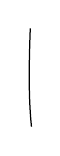
\begin{tikzpicture}[x=1cm,y=1cm]
\draw[line width=.45pt] (0,1.25) .. controls (-.015,.82) and (-.025,.40) .. (.015,0);
\end{tikzpicture}}

To show this, we shall embed
$\Pi_{0,3}$ as a subgroup of finite index
in $\Pi'_{0,3}$, whence an \LMsourceMark{M000085}{\unsure{analogous}} embedding
\var{\deleted{\LMsourceMark{M000086}{\illegible{1}}}}{\LMsourceMark{M000087}{\LMcancelledDoubts{\LMsourceMark{M000088}{\illegible{1}}}}}{deletion}{140-2-s506-D003}
\[
(2)\qquad\widehat{\Pi}_{0,3}\lhook\joinrel\longrightarrow\widehat{\Pi}'_{0,3}
\]
which will be compatible with the outer action of $\Gamma$.

\LMflushnotes\LMflushpages
\ifnum\LMform=1
\begin{LMapparatus}
\LMentry{140-2-s506-I001}{insertion}{\inserted{for triangulated structures}
}{\emph{\LMinsertedlabel}}{Explicit authorial insertion: integrated at the position recorded by the transcription, without changing its reading.}{}
\LMentry{140-2-s506-D001}{deletion}{\deleted{whose}
}{\emph{\LMomittedlabel}}{Cancelled in the manuscript: omission follows the author's final state; uncertainty in the cancelled material remains marked.}{}
\LMentry{140-2-s506-D002}{deletion}{\deleted{on which}
}{\emph{\LMomittedlabel}}{Cancelled in the manuscript: omission follows the author's final state; uncertainty in the cancelled material remains marked.}{}
\LMentry{140-2-s506-D003}{deletion}{\deleted{\LMsourceMark{M000089}{\illegible{1}}}
}{\emph{\LMomittedlabel}}{Cancelled in the manuscript: omission follows the author's final state; uncertainty in the cancelled material remains marked.}{}
\end{LMapparatus}
\fi
\ifnum\LMform=2
\par\smallskip\begingroup\footnotesize\noindent\textcolor{gray}{\rule{.2\linewidth}{.35pt}}\par
\noindent\textit{\LMdoubtheading.}\par
\LMcarryover{140-2-s506-D003}{\LMsourceMark{M000090}{\illegible{1}}
}
\par\endgroup\smallskip
\fi

\LMsourceMark{M000091}{\scanpage{507}}

For this, consider the quotient scheme
\[
Y=\underbrace{\mathbb P^1_{\mathbb Q}}_{X}/\LMsourceMark{M000092}{\unsure{\mathfrak S_3}}
\]
with the three points \var{\inserted{$a_0,a_1,a_\infty$}}{\LMadded{$a_0,a_1,a_\infty$}}{insertion}{140-2-s507-I001} of $Y$, rational over
$\mathbb Q$, \var{\inserted{$a_0$}}{\LMadded{$a_0$}}{insertion}{140-2-s507-I002} corresponding to the orbit
\var{\deleted{of the}}{}{deletion}{140-2-s507-D001} $\{0,1,\infty\}$, $a_1$ to the orbit
$\{-1,\frac12,2\}$, and $a_\infty$ to the orbit
$\{\LMsourceMark{M000093}{\unsure{-j}},\LMsourceMark{M000094}{\unsure{-\overline j}}\}$ of $\LMsourceMark{M000095}{\unsure{\mathfrak S_3}}$
\LMsourceMark{M000096}{\margin{$j=\exp\frac{2i\pi}{3}$}}
(which exhausts \LMsourceMark{M000097}{\unsure{the set}} of geometric
``singular'' orbits). We know that $Y$ is a projective line
(over $\overline{\mathbb Q}$ a priori), \LMsourceMark{M000098}{\unsure{which we}} \LMsourceMark{M000099}{\unsure{pin}} by
$a_0,a_1,a_\infty$ as points $0,1,\infty$, \LMsourceMark{M000100}{\unsure{(thus}}
$Y\simeq\mathbb P^1_{\mathbb Q}$ -- the \var{\deleted{\LMsourceMark{M000101}{\illegible{1}}}}{\LMsourceMark{M000102}{\LMcancelledDoubts{\LMsourceMark{M000103}{\illegible{1}}}}}{deletion}{140-2-s507-D002} morphism
$X\longrightarrow Y$ is thus identified with a well-determined morphism
\[
(3)\qquad
f:\begin{array}{ccc}
\mathbb P^1_{\mathbb Q}&\longrightarrow&\mathbb P^1_{\mathbb Q}\\
\Vert&&\Vert\\
X&&Y
\end{array}
\]
\var{\deleted{(in fact, $f$ can be defined as a morphism
$\mathbb P^1_{\mathbb Z}\longrightarrow\mathbb P^1_{\mathbb Z}$,
but here this matters little to us)}}{}{deletion}{140-2-s507-D003}
which makes $X$ a Galois \LMsourceMark{M000104}{\unsure{covering|covering}} of $Y$, with group
$\LMsourceMark{M000105}{\unsure{\mathfrak S_3}}$, étale \LMsourceMark{M000106}{\unsure{over|over}}
$\mathbb P^1_{\mathbb Q}\setminus\{0,1,\infty\}$, with ramification
indices at these points $2,2,3$. From the point of view of the geometry of maps
(\LMsourceMark{M000107}{\unsure{placing oneself|immersing oneself}} over the base field $\mathbb C$), we consider the

\LMflushnotes\LMflushpages
\ifnum\LMform=1
\begin{LMapparatus}
\LMentry{140-2-s507-I001}{insertion}{\inserted{$a_0,a_1,a_\infty$}
}{\emph{\LMinsertedlabel}}{Explicit authorial insertion: integrated at the position recorded by the transcription, without changing its reading.}{}
\LMentry{140-2-s507-I002}{insertion}{\inserted{$a_0$}
}{\emph{\LMinsertedlabel}}{Explicit authorial insertion: integrated at the position recorded by the transcription, without changing its reading.}{}
\LMentry{140-2-s507-D001}{deletion}{\deleted{of the}
}{\emph{\LMomittedlabel}}{Cancelled in the manuscript: omission follows the author's final state; uncertainty in the cancelled material remains marked.}{}
\LMentry{140-2-s507-D002}{deletion}{\deleted{\LMsourceMark{M000108}{\illegible{1}}}
}{\emph{\LMomittedlabel}}{Cancelled in the manuscript: omission follows the author's final state; uncertainty in the cancelled material remains marked.}{}
\LMentry{140-2-s507-D003}{deletion}{\deleted{(in fact, $f$ can be defined as a morphism
$\mathbb P^1_{\mathbb Z}\longrightarrow\mathbb P^1_{\mathbb Z}$,
but here this matters little to us)}
}{\emph{\LMomittedlabel}}{Cancelled in the manuscript: omission follows the author's final state; uncertainty in the cancelled material remains marked.}{}
\end{LMapparatus}
\fi
\ifnum\LMform=2
\par\smallskip\begingroup\footnotesize\noindent\textcolor{gray}{\rule{.2\linewidth}{.35pt}}\par
\noindent\textit{\LMdoubtheading.}\par
\LMcarryover{140-2-s507-D002}{\LMsourceMark{M000109}{\illegible{1}}
}
\par\endgroup\smallskip
\fi

\LMsourceMark{M000110}{\scanpage{508}}
\LMsourceMark{M000111}{\mspage{\LMsourceMark{M000112}{\unsure{258 (259)}}}}

map determined on $X$ by the spherical triangles $(0,1,\infty)$
(on the real axis as equator) -- which is thus the universal
\LMsourceMark{M000113}{\unsure{weighted}} triangular map -- as the inverse image of the universal map
(having a single vertex $0$, a single edge (folded) $0\longrightarrow1$,
a single face, with center $\infty$).
\LMsourceMark{M000114}{\margin{\figure{\begin{tikzpicture}[x=1cm,y=1cm,line cap=round,line join=round]
\draw[line width=.45pt] (0,2.85)
 .. controls (-.71,2.83) and (-1.02,2.47) .. (-1,2)
 .. controls (-1.01,1.48) and (-.57,1.16) .. (0,1.15);
\draw[line width=.45pt] (0,2.85)
 .. controls (.76,2.85) and (1.03,2.48) .. (1,2.10);
\draw[line width=.45pt] (.99,1.98)
 .. controls (.98,1.62) and (.74,1.36) .. (.54,1.26);
\draw[line width=.5pt] (-1,2)
 .. controls (-.91,1.75) and (.83,1.74) .. (1,1.95);
\draw[densely dotted,line width=.65pt] (-1,2)
 .. controls (-.61,2.17) and (.63,2.17) .. (1,2.02);
\fill (0,2.85) circle (1.4pt);
\node[anchor=south west,inner sep=2pt] at (0,2.88) {$P=\LMsourceMark{M000115}{\unsure{-\bar j|-j}}$};
\fill (0,1.15) circle (1.4pt);
\node[anchor=north west,inner sep=2pt] at (-.03,1.12) {$P'=\LMsourceMark{M000116}{\unsure{-j|-\bar j}}$};
\fill (-.57,1.80) circle (1.4pt);
\node[below,inner sep=2pt] at (-.57,1.80) {$0$};
\fill (.78,1.82) circle (1.4pt);
\node[below,inner sep=2pt] at (.78,1.82) {$1$};
\fill (0,2.12) circle (1.5pt);
\node[above,inner sep=2pt] at (0,2.12) {$\infty$};
\draw[->,line width=.65pt] (-1.40,1.60)
 .. controls (-1.40,1.22) and (-1.38,.85) .. (-1.37,.58);
\draw[line width=.45pt] (.02,.48)
 .. controls (-.55,.48) and (-.86,.17) .. (-.82,-.20)
 .. controls (-.78,-.70) and (-.46,-1.02) .. (.10,-1.04);
\draw[line width=.45pt] (.02,.48)
 .. controls (.65,.46) and (.87,.12) .. (.82,-.29)
 .. controls (.81,-.58) and (.66,-.79) .. (.53,-.87);
\fill (.02,.48) circle (1.5pt);
\node[anchor=west,inner sep=2pt] at (.07,.48) {$\LMsourceMark{M000117}{\unsure{Q}}(=P)$};
\fill (-.82,-.12) circle (1.5pt);
\node[left,inner sep=2pt] at (-.82,-.12) {$\infty$};
\fill (-.08,.10) circle (1.7pt);
\node[below,inner sep=2pt] at (-.08,.10) {$1$};
\fill (-.40,-.36) circle (1.7pt);
\node[below,inner sep=2pt] at (-.40,-.36) {$0$};
\draw[line width=1.15pt] (-.08,.10)
 .. controls (.28,.10) and (.71,.02) .. (.82,-.20)
 .. controls (.66,-.43) and (.03,-.47) .. (-.40,-.36);
\draw[densely dotted,line width=.65pt] (-.82,-.12)
 .. controls (-.60,.08) and (-.36,.08) .. (-.08,.10);
\draw[densely dotted,line width=.65pt] (-.82,-.12)
 .. controls (-.78,-.32) and (-.59,-.35) .. (-.40,-.36);
\node[below,inner sep=1pt] at (.22,-.44) {$\LMsourceMark{M000118}{\unsure{\varphi}}$};
\end{tikzpicture}}}}
Every topological \var{\deleted{\LMsourceMark{M000119}{\unsure{of}}}}{\LMsourceMark{M000120}{\LMcancelledDoubts{\LMsourceMark{M000121}{\unsure{of}}}}}{deletion}{140-2-s508-D001} \var{\inserted{étale}}{\LMadded{étale}}{insertion}{140-2-s508-I001} covering of
$U_{03}(\mathbb C)\subset X$ thus gives a topological étale covering of
$U_{0,3}(\mathbb C)\subset Y$, \var{\deleted{ramified}}{}{deletion}{140-2-s508-D002} having
\var{\deleted{\LMsourceMark{M000122}{\illegible{1}}}}{\LMsourceMark{M000123}{\LMcancelledDoubts{\LMsourceMark{M000124}{\illegible{1}}}}}{deletion}{140-2-s508-D003} \var{\inserted{over}}{\LMadded{over}}{insertion}{140-2-s508-I002} $1$ ramification $2$,
over $\infty$ ramification $3$ \LMsourceMark{M000125}{\unsure{exactly|exactly}},
which corresponds to the ``forgetful'' functor \var{\inserted{(of the weighting)}}{\LMadded{(of the weighting)}}{insertion}{140-2-s508-I003},
where a \LMsourceMark{M000126}{\unsure{weighted}} triangular map is considered as
just a map. From the point of view of fundamental groups \LMsourceMark{M000127}{\unsure{we}} thus find
an \var{\deleted{\LMsourceMark{M000128}{\unsure{homomorphism}} of outer groups}}{\LMsourceMark{M000129}{\LMcancelledDoubts{\LMsourceMark{M000130}{\unsure{homomorphism}}}}}{deletion}{140-2-s508-D004}
\var{\inserted{equivalence of categories}}{\LMadded{equivalence of categories}}{insertion}{140-2-s508-I004}

\diagram{\begin{tikzcd}[ampersand replacement=\&,column sep=large,row sep=huge,column sep=9pt,row sep=14pt,execute at begin picture={\fontsize{10}{12}\selectfont},nodes in empty cells]
\&
\var{\deleted{\begin{gathered}
\Pi_1(\LMsourceMark{M000131}{\unsure{X(\mathbb C)}}\setminus\{0,1,\infty\})\\[-2pt]
\rotatebox{90}{$=$}\\[-2pt]
\Pi_{0,3}
\end{gathered}}}{\LMsourceMark{M000132}{\LMcancelledDoubts{\(\LMsourceMark{M000133}{\unsure{X(\mathbb C)}}\)}}}{deletion}{140-2-s508-D005}
\arrow[r,phantom,"{\var{\deleted{\longleftarrow}}{}{deletion}{140-2-s508-D006}}" description]
\&
\var{\deleted{\begin{gathered}
\Pi_1\!\left(Y(\mathbb C)\setminus\{0,1,\infty\};
\underbrace{2\{1\}+3\{\infty\}}_{\substack{\text{signature of}\\\text{ramification}}}\right)\\[-2pt]
\rotatebox{90}{$=$}\\[-2pt]
\Pi'_{0,3}
\end{gathered}}}{}{deletion}{140-2-s508-D007}
\\
(\var{\deleted{\LMsourceMark{M000134}{\illegible{1}}}}{\LMsourceMark{M000135}{\LMcancelledDoubts{\(\LMsourceMark{M000136}{\illegible{1}}\)}}}{deletion}{140-2-s508-D008}\var{\inserted{4}}{\LMadded{4}}{insertion}{140-2-s508-I005}) \&
\left(\text{Étale coverings of }X\setminus\{0,1,\infty\}=U_{0,3}\right)
\arrow[r,phantom,"\simeq" description]
\arrow[d,phantom,"{\rotatebox{-90}{$\simeq$}}" description]
\&
\begin{gathered}
\left[\begin{gathered}
\text{Coverings of }Y\setminus\{0,1,\infty\}=U_{0,3}\\
\text{with ramification subordinate to}\\
\text{the signature }2\{1\}+3\{\infty\}
\end{gathered}\right]\\
\big/\begin{gathered}
\text{the object }(X\setminus\{0,1,\infty\})\\
\text{of the said category}
\end{gathered}
\end{gathered}
\arrow[d,phantom,"{\rotatebox{90}{$\simeq$}}" description]
\\
\& \Pi_{0,3}\text{-sets} \&
(\Pi'_{0,3}\text{-Sets})/\var{\deleted{\LMsourceMark{M000137}{\unsure{E}}}}{\LMsourceMark{M000138}{\LMcancelledDoubts{\(\LMsourceMark{M000139}{\unsure{E}}\)}}}{deletion}{140-2-s508-D009}E
\end{tikzcd}}

where $E$ is the $\Pi'_{0,3}$-set corresponding to the object
$X\setminus\{0,1,\infty\}$ of the category of étale coverings of
$\LMsourceMark{M000140}{\unsure{Y\setminus\{0,1,\infty\}}}$ with ramification
\var{\deleted{\LMsourceMark{M000141}{\unsure{imposed}}}}{\LMsourceMark{M000142}{\LMcancelledDoubts{\LMsourceMark{M000143}{\unsure{imposed}}}}}{deletion}{140-2-s508-D010}\var{\inserted{\LMsourceMark{M000144}{\unsure{subordin-}}}}{\LMadded{\LMsourceMark{M000145}{\unsure{subordin-}}}}{insertion}{140-2-s508-I006}ate to
$2\{1\}+3\{\infty\}$

\var{\deleted{$\LMsourceMark{M000146}{\unsure{\simeq}}\ \LMsourceMark{M000147}{\unsure{\Pi_{0,3}^{\prime\circ}}}\in\mathrm{Ens}$}}{\LMsourceMark{M000148}{\LMcancelledDoubts{\(\LMsourceMark{M000149}{\unsure{\simeq}}\)\quad \(\LMsourceMark{M000150}{\unsure{\Pi_{0,3}^{\prime\circ}}}\)}}}{deletion}{140-2-s508-D011}

\LMflushnotes\LMflushpages
\ifnum\LMform=1
\begin{LMapparatus}
\LMentry{140-2-s508-D001}{deletion}{\deleted{\LMsourceMark{M000151}{\unsure{of}}}
}{\emph{\LMomittedlabel}}{Cancelled in the manuscript: omission follows the author's final state; uncertainty in the cancelled material remains marked.}{}
\LMentry{140-2-s508-I001}{insertion}{\inserted{étale}
}{\emph{\LMinsertedlabel}}{Explicit authorial insertion: integrated at the position recorded by the transcription, without changing its reading.}{}
\LMentry{140-2-s508-D002}{deletion}{\deleted{ramified}
}{\emph{\LMomittedlabel}}{Cancelled in the manuscript: omission follows the author's final state; uncertainty in the cancelled material remains marked.}{}
\LMentry{140-2-s508-D003}{deletion}{\deleted{\LMsourceMark{M000152}{\illegible{1}}}
}{\emph{\LMomittedlabel}}{Cancelled in the manuscript: omission follows the author's final state; uncertainty in the cancelled material remains marked.}{}
\LMentry{140-2-s508-I002}{insertion}{\inserted{over}
}{\emph{\LMinsertedlabel}}{Explicit authorial insertion: integrated at the position recorded by the transcription, without changing its reading.}{}
\LMentry{140-2-s508-I003}{insertion}{\inserted{(of the weighting)}
}{\emph{\LMinsertedlabel}}{Explicit authorial insertion: integrated at the position recorded by the transcription, without changing its reading.}{}
\LMentry{140-2-s508-D004}{deletion}{\deleted{\LMsourceMark{M000153}{\unsure{homomorphism}} of outer groups}
}{\emph{\LMomittedlabel}}{Cancelled in the manuscript: omission follows the author's final state; uncertainty in the cancelled material remains marked.}{}
\LMentry{140-2-s508-I004}{insertion}{\inserted{equivalence of categories}
}{\emph{\LMinsertedlabel}}{Explicit authorial insertion: integrated at the position recorded by the transcription, without changing its reading.}{}
\LMentry{140-2-s508-D005}{deletion}{\(\deleted{\begin{gathered}
\Pi_1(\LMsourceMark{M000154}{\unsure{X(\mathbb C)}}\setminus\{0,1,\infty\})\\[-2pt]
\rotatebox{90}{$=$}\\[-2pt]
\Pi_{0,3}
\end{gathered}}\)
}{\emph{\LMomittedlabel}}{Cancelled in the manuscript: omission follows the author's final state; uncertainty in the cancelled material remains marked.}{}
\LMentry{140-2-s508-D006}{deletion}{\(\deleted{\longleftarrow}\)
}{\emph{\LMomittedlabel}}{Cancelled in the manuscript: omission follows the author's final state; uncertainty in the cancelled material remains marked.}{}
\LMentry{140-2-s508-D007}{deletion}{\(\deleted{\begin{gathered}
\Pi_1\!\left(Y(\mathbb C)\setminus\{0,1,\infty\};
\underbrace{2\{1\}+3\{\infty\}}_{\substack{\text{signature of}\\\text{ramification}}}\right)\\[-2pt]
\rotatebox{90}{$=$}\\[-2pt]
\Pi'_{0,3}
\end{gathered}}\)
}{\emph{\LMomittedlabel}}{Cancelled in the manuscript: omission follows the author's final state; uncertainty in the cancelled material remains marked.}{}
\LMentry{140-2-s508-D008}{deletion}{\(\deleted{\LMsourceMark{M000155}{\illegible{1}}}\)
}{\emph{\LMomittedlabel}}{Cancelled in the manuscript: omission follows the author's final state; uncertainty in the cancelled material remains marked.}{}
\LMentry{140-2-s508-I005}{insertion}{\(\inserted{4}\)
}{\emph{\LMinsertedlabel}}{Explicit authorial insertion: integrated at the position recorded by the transcription, without changing its reading.}{}
\LMentry{140-2-s508-D009}{deletion}{\(\deleted{\LMsourceMark{M000156}{\unsure{E}}}\)
}{\emph{\LMomittedlabel}}{Cancelled in the manuscript: omission follows the author's final state; uncertainty in the cancelled material remains marked.}{}
\LMentry{140-2-s508-D010}{deletion}{\deleted{\LMsourceMark{M000157}{\unsure{imposed}}}
}{\emph{\LMomittedlabel}}{Cancelled in the manuscript: omission follows the author's final state; uncertainty in the cancelled material remains marked.}{}
\LMentry{140-2-s508-I006}{insertion}{\inserted{\LMsourceMark{M000158}{\unsure{subordin-}}}
}{\emph{\LMinsertedlabel}}{Explicit authorial insertion: integrated at the position recorded by the transcription, without changing its reading.}{}
\LMentry{140-2-s508-D011}{deletion}{\deleted{$\LMsourceMark{M000159}{\unsure{\simeq}}\ \LMsourceMark{M000160}{\unsure{\Pi_{0,3}^{\prime\circ}}}\in\mathrm{Ens}$}
}{\emph{\LMomittedlabel}}{Cancelled in the manuscript: omission follows the author's final state; uncertainty in the cancelled material remains marked.}{}
\end{LMapparatus}
\fi
\ifnum\LMform=2
\par\smallskip\begingroup\footnotesize\noindent\textcolor{gray}{\rule{.2\linewidth}{.35pt}}\par
\noindent\textit{\LMdoubtheading.}\par
\LMcarryover{140-2-s508-D001}{\LMsourceMark{M000161}{\unsure{of}}
}
\LMcarryover{140-2-s508-D003}{\LMsourceMark{M000162}{\illegible{1}}
}
\LMcarryover{140-2-s508-D004}{\LMsourceMark{M000163}{\unsure{homomorphism}}
}
\LMcarryover{140-2-s508-D005}{\(\LMsourceMark{M000164}{\unsure{X(\mathbb C)}}\)
}
\LMcarryover{140-2-s508-D008}{\(\LMsourceMark{M000165}{\illegible{1}}\)
}
\LMcarryover{140-2-s508-D009}{\(\LMsourceMark{M000166}{\unsure{E}}\)
}
\LMcarryover{140-2-s508-D010}{\LMsourceMark{M000167}{\unsure{imposed}}
}
\LMcarryover{140-2-s508-D011}{\(\LMsourceMark{M000168}{\unsure{\simeq}}\)\quad \(\LMsourceMark{M000169}{\unsure{\Pi_{0,3}^{\prime\circ}}}\)
}
\par\endgroup\smallskip
\fi

\LMsourceMark{M000170}{\scanpage{509}}
\LMsourceMark{M000171}{\mspage{\LMsourceMark{M000172}{\unsure{260|250}}}}

Here, \var{\deleted{\LMsourceMark{M000173}{\illegible{3}}}}{\LMsourceMark{M000174}{\LMcancelledDoubts{\LMsourceMark{M000175}{\illegible{3}}}}}{deletion}{140-2-s509-D001} \var{\inserted{\deleted{\LMsourceMark{M000176}{\illegible{1}}} the base point of $Y-\{0,1,\infty\}$ chosen\LMsourceMark{M000177}{\unsure{;|,}} \LMsourceMark{M000178}{\unsure{to}} describe the}}{\LMadded{\var{\deleted{\LMsourceMark{M000179}{\illegible{1}}}}{\LMsourceMark{M000180}{\LMcancelledDoubts{\LMsourceMark{M000181}{\illegible{1}}}}}{deletion}{140-2-s509-D002} the base point of $Y-\{0,1,\infty\}$ chosen\LMsourceMark{M000182}{\unsure{;|,}} \LMsourceMark{M000183}{\unsure{to}} describe the}}{insertion}{140-2-s509-I001} coverings \var{\deleted{$E=\LMsourceMark{M000184}{\unsure{f^{-1}}}\LMsourceMark{M000185}{\unsure{(}}$}}{\LMsourceMark{M000186}{\LMcancelledDoubts{\(\LMsourceMark{M000187}{\unsure{f^{-1}}}\)\quad \(\LMsourceMark{M000188}{\unsure{(}}\)}}}{deletion}{140-2-s509-D003} (with ramification \LMsourceMark{M000189}{\unsure{subordinate}} to \dots) by a fundamental group with ramification, being \LMsourceMark{M000190}{\unsure{again}} $P=-\bar j$, we shall have
\[
(5)\qquad E=f_{\LMsourceMark{M000191}{\unsure{\mathbf C|\mathbb C}}}^{-1}(P)
\]
and we can thus make explicit the category $(\Pi'_{03}\text{-Sets})/E$\LMsourceMark{M000192}{\unsure{;}}

Where $E$ is a homogeneous space, \var{\inserted{\LMsourceMark{M000193}{\unsure{isomorphic to the}}}}{\LMadded{\LMsourceMark{M000194}{\unsure{isomorphic to the}}}}{insertion}{140-2-s509-I002} \LMsourceMark{M000195}{\unsure{quotient}} of $\Pi'_{03}$ by the \LMsourceMark{M000196}{\unsure{subgroup|subgroup}} \var{\inserted{$\Pi'^{\circ}_{03}$}}{\LMadded{$\Pi'^{\circ}_{03}$}}{insertion}{140-2-s509-I003} kernel of the \var{\inserted{suitable}}{\LMadded{suitable}}{insertion}{140-2-s509-I004} surjective homomorphism
\[
(6)\qquad
\left\{
\begin{array}{l}
\Pi'_{0,3}\longrightarrow\LMsourceMark{M000197}{\unsure{\mathfrak S_3|\mathcal S_3}}\\[2pt]
\left.
\begin{array}{lll}
\ell_0 &\longmapsto& \text{element of order 2}\\
\ell_1 &\longmapsto& \text{element of order 2}\\
\ell_\infty &\longmapsto& \text{\LMsourceMark{M000198}{\unsure{element}} of order 3}
\end{array}
\right)\quad\text{to be computed !}
\end{array}
\right.
\]

We choose a $Q_0\in E$ as ``origin'' of $E$ -- so as to be able to identify $E$ as a $\Pi'_{0,3}$-set with $\Pi'_{03}/\Pi'^{\circ}_{03}\simeq\LMsourceMark{M000199}{\unsure{\mathfrak S_3}}$ -- then $(\mathrm{Ens}\,\Pi'_{03})/E$ is identified, by the functor $F\longmapsto F_{Q_0}$, with $\mathrm{Ens}(\Pi'^{\circ}_{03})$.

We thus find in summary an equivalence of categories (depending on the choice of $Q_0$)
\[
\Pi_{03}\text{-sets}\quad\LMsourceMark{M000200}{\unsure{\simeq}}\quad\Pi'^{\circ}_{03}\text{-sets}
\]
which is itself described by a bitorsor under $(\Pi'^{\circ}_{0,3},\Pi_{03})$ -- and, up to isomorphism \var{\deleted{that}}{}{deletion}{140-2-s509-D004} (not unique !), by an isomorphism
\[
\Pi_{03}\simeq\Pi'^{\circ}_{0,3}\quad -
\]
the isomorphisms thus obtained (for

\LMflushnotes\LMflushpages
\ifnum\LMform=1
\begin{LMapparatus}
\LMentry{140-2-s509-D001}{deletion}{\deleted{\LMsourceMark{M000201}{\illegible{3}}}
}{\emph{\LMomittedlabel}}{Cancelled in the manuscript: omission follows the author's final state; uncertainty in the cancelled material remains marked.}{}
\LMentry{140-2-s509-I001}{insertion}{\inserted{\deleted{\LMsourceMark{M000202}{\illegible{1}}} the base point of $Y-\{0,1,\infty\}$ chosen\LMsourceMark{M000203}{\unsure{;|,}} \LMsourceMark{M000204}{\unsure{to}} describe the}
}{\emph{\LMinsertedlabel}}{Explicit authorial insertion: integrated at the position recorded by the transcription, without changing its reading.}{}
\LMentry{140-2-s509-D002}{deletion}{\deleted{\LMsourceMark{M000205}{\illegible{1}}}
}{\emph{\LMomittedlabel}}{Cancelled in the manuscript: omission follows the author's final state; uncertainty in the cancelled material remains marked.}{}
\LMentry{140-2-s509-D003}{deletion}{\deleted{$E=\LMsourceMark{M000206}{\unsure{f^{-1}}}\LMsourceMark{M000207}{\unsure{(}}$}
}{\emph{\LMomittedlabel}}{Cancelled in the manuscript: omission follows the author's final state; uncertainty in the cancelled material remains marked.}{}
\LMentry{140-2-s509-I002}{insertion}{\inserted{\LMsourceMark{M000208}{\unsure{isomorphic to the}}}
}{\emph{\LMinsertedlabel}}{Explicit authorial insertion: integrated at the position recorded by the transcription, without changing its reading.}{}
\LMentry{140-2-s509-I003}{insertion}{\inserted{$\Pi'^{\circ}_{03}$}
}{\emph{\LMinsertedlabel}}{Explicit authorial insertion: integrated at the position recorded by the transcription, without changing its reading.}{}
\LMentry{140-2-s509-I004}{insertion}{\inserted{suitable}
}{\emph{\LMinsertedlabel}}{Explicit authorial insertion: integrated at the position recorded by the transcription, without changing its reading.}{}
\LMentry{140-2-s509-D004}{deletion}{\deleted{that}
}{\emph{\LMomittedlabel}}{Cancelled in the manuscript: omission follows the author's final state; uncertainty in the cancelled material remains marked.}{}
\end{LMapparatus}
\fi
\ifnum\LMform=2
\par\smallskip\begingroup\footnotesize\noindent\textcolor{gray}{\rule{.2\linewidth}{.35pt}}\par
\noindent\textit{\LMdoubtheading.}\par
\LMcarryover{140-2-s509-D001}{\LMsourceMark{M000209}{\illegible{3}}
}
\LMcarryover{140-2-s509-D002}{\LMsourceMark{M000210}{\illegible{1}}
}
\LMcarryover{140-2-s509-D003}{\(\LMsourceMark{M000211}{\unsure{f^{-1}}}\)\quad \(\LMsourceMark{M000212}{\unsure{(}}\)
}
\par\endgroup\smallskip
\fi

\LMsourceMark{M000213}{\scanpage{510}}
\LMsourceMark{M000214}{\mspage{\LMsourceMark{M000215}{\unsure{249}}}}

varying origins of the bitorsor) \LMsourceMark{M000216}{\unsure{form|forming}} exactly a conjugacy class under $\Pi'^{\circ}_{03}$ -- i.e. an \uline{outer} \uline{\LMsourceMark{M000217}{\unsure{isomorphism}}} $\Pi_{03}\simeq\Pi'^{\circ}_{03}$. When in addition the choice of $Q_0$ varies, we find \var{\deleted{as}}{}{deletion}{140-2-s510-D001} a \LMsourceMark{M000218}{\unsure{composite|composites}}
\[
\Pi_{0,3}\longrightarrow\Pi'^{\circ}_{03}\longrightarrow\Pi'_{03}
\]
\var{\deleted{\LMsourceMark{M000219}{\unsure{exactly}}}}{\LMsourceMark{M000220}{\LMcancelledDoubts{\LMsourceMark{M000221}{\unsure{exactly}}}}}{deletion}{140-2-s510-D002} a $\Pi'_{03}$-conjugacy class, i.e. an outer homomorphism.

I have \LMsourceMark{M000222}{\unsure{slaved away}} a lot for not much -- for lack of having written down the \LMsourceMark{M000223}{\unsure{necessary|elementary}} \var{\inserted{general}}{\LMadded{general}}{insertion}{140-2-s510-I001} \LMsourceMark{M000224}{\unsure{functorialities}} for ``fundamental groups \LMsourceMark{M000225}{\unsure{with}} ramification''. \LMsourceMark{M000226}{\unsure{For example}} the mysterious bifunctor $I$ from earlier is made up of \LMsourceMark{M000227}{\unsure{classes}} of paths from $P\in\LMsourceMark{M000228}{\unsure{X(\mathbb C)|X_{\mathbb C}}}\setminus\{0,1,\infty\}$ (base point for computing $\Pi_{0,3}$) to $Q_0$ (playing the role of a new base point, having the merit of mapping to the one \var{\inserted{-- $P$ --}}{\LMadded{-- $P$ --}}{insertion}{140-2-s510-I002} which serves to compute $\Pi'_{03}$, fundamental group with ramification on $Y(\mathbb C)\setminus\{0,1,\infty\}$ \dots) It would perhaps be more convenient to define \LMsourceMark{M000229}{\unsure{direct\textsuperscript{ly}|directly}} a functor in the opposite direction\LMsourceMark{M000230}{\unsure{:|.}}
\[
(7)\qquad
\begin{array}{c}
\text{Coverings of }Y(\mathbb C)\var{\inserted{\setminus(0,1,\infty)}}{\LMadded{\setminus(0,1,\infty)}}{insertion}{140-2-s510-I003}\ \text{subordinate}\\
\text{to the signature }2\{1\}+3\{\infty\}
\end{array}
\longrightarrow
\begin{array}{c}
\text{\LMsourceMark{M000231}{\unsure{Étale|Étale}} coverings of}\\
X(\mathbb C)\setminus\{0,1,\infty\}
\end{array}
\]
by inverse image, \LMsourceMark{M000232}{\unsure{followed|followed}} by a \uline{normalization}

\LMflushnotes\LMflushpages
\ifnum\LMform=1
\begin{LMapparatus}
\LMentry{140-2-s510-D001}{deletion}{\deleted{as}
}{\emph{\LMomittedlabel}}{Cancelled in the manuscript: omission follows the author's final state; uncertainty in the cancelled material remains marked.}{}
\LMentry{140-2-s510-D002}{deletion}{\deleted{\LMsourceMark{M000233}{\unsure{exactly}}}
}{\emph{\LMomittedlabel}}{Cancelled in the manuscript: omission follows the author's final state; uncertainty in the cancelled material remains marked.}{}
\LMentry{140-2-s510-I001}{insertion}{\inserted{general}
}{\emph{\LMinsertedlabel}}{Explicit authorial insertion: integrated at the position recorded by the transcription, without changing its reading.}{}
\LMentry{140-2-s510-I002}{insertion}{\inserted{-- $P$ --}
}{\emph{\LMinsertedlabel}}{Explicit authorial insertion: integrated at the position recorded by the transcription, without changing its reading.}{}
\LMentry{140-2-s510-I003}{insertion}{\(\inserted{\setminus(0,1,\infty)}\)
}{\emph{\LMinsertedlabel}}{Explicit authorial insertion: integrated at the position recorded by the transcription, without changing its reading.}{}
\end{LMapparatus}
\fi
\ifnum\LMform=2
\par\smallskip\begingroup\footnotesize\noindent\textcolor{gray}{\rule{.2\linewidth}{.35pt}}\par
\noindent\textit{\LMdoubtheading.}\par
\LMcarryover{140-2-s510-D002}{\LMsourceMark{M000234}{\unsure{exactly}}
}
\par\endgroup\smallskip
\fi

% END PACKAGE LM_P051
\end{document}
